\let\lesson\undefined
\newcommand{\lesson}{\phantomlesson{Bài 8: Áp suất - Động năng chất khí theo mô hình động học phân tử}}
\chapter[Áp suất - Động năng chất khí theo mô hình động học phân tử]{Áp suất - Động năng chất khí theo mô hình động học phân tử}
\section{Lý thuyết}
\subsection{Áp suất chất khí theo mô hình động học phân tử}
Áp suất khí tác dụng lên thành bình càng tăng khi các phân tử khí chuyển động nhiệt càng nhanh, khối lượng và mật độ phân tử khí càng lớn.\\
Biểu thức áp suất chất khí tác dụng lên thành bình:
\begin{equation}
	p=\dfrac{1}{3}\mu m\overline{v^2}
\end{equation}
Trong đó:
\begin{itemize}
	\item $p$: áp suất khí, đơn vị trong hệ SI là $\si{\pascal}$;
	\item $m$: khối lượng của mỗi phân tử khí, đơn vị trong hệ SI là $\si{\kilogram}$;
	\item $\mu$: mật độ phân tử khí, đơn vị trong hệ SI là $\si{\meter^{-3}}$;
	\item $\overline{v^2}$: trung bình của bình phương tốc độ chuyển động nhiệt của mỗi phân tử khí, đơn vị trong hệ SI là $\si{\meter^2/\second^2}$.
\end{itemize}
\luuy{Căn bậc hai của $\overline{v^2}$ là $\sqrt{\overline{v^2}}$, độ lớn của đại lượng này không phải là tốc độ trung bình của các phân tử. Nó được gọi là \textit{tốc độ căn quân phương} của phân tử.
}
\subsection{Động năng tịnh tiến trung bình của phân tử khí}
Động năng tịnh tiến trung bình của phân tử khí tỉ lệ với nhiệt độ tuyệt đối của khí:
\begin{equation}
	W_\text{đ}=\dfrac{3}{2}kT
\end{equation}
Trong đó, hằng số Boltzmann $k$ là hằng số khí đặc trưng cho mối liên hệ giữa nhiệt độ và năng lượng. Giá trị của hằng số Boltzmann trong hệ SI bằng
$$k=\dfrac{R}{N_A}\approx\SI{1.38E-23}{\joule/\kelvin}.$$
\manatip{Có thể biểu diễn sự phụ thuộc của áp suất theo nhiệt độ tuyệt đối $T$ và mật độ phân tử khí $n$:
$$pV=\dfrac{N}{N_\text{A}}RT\Rightarrow p=\dfrac{N}{V}\cdot\dfrac{R}{N_\text{A}}\cdot T=\mu kT.$$
Hay
$$p=\dfrac{2}{3}\mu W_\text{đ}.$$}
\section{Mục tiêu bài học - Ví dụ minh hoạ}
\begin{dang}{Giải thích được chuyển động của các phân tử ảnh hưởng như thế nào đến áp suất tác dụng lên thành bình và từ đó rút ra được hệ thức $p=\dfrac{1}{3}\mu m\overline{v^2}$.}
	\viduii{3}
	{Trong bài tập này, chúng ta sẽ chứng minh lại những điều được học trong phần lý thuyết.
		\begin{enumerate}[label=\alph*)]
			\item Em hãy giải thích vì sao áp suất do các phân tử khí tác dụng lên thành bình phụ thuộc vào tốc độ chuyển động nhiệt, khối lượng và mật độ của các phân tử khí?
			\item Bây giờ, ta xét mô hình va chạm một chiều đơn giản: Hệ gồm các phân tử khí khối lượng $m$ chuyển động dọc theo trục $Ox$ với tốc độ $v_x$ đến va chạm đàn hồi với thành bình rồi bật ngược trở lại với cùng tốc độ ban đầu. Trong thời gian va chạm $\Delta t$, số phân tử đập vào diện tích $S$ của thành bình là số phân tử chứa trong một hình trụ đáy $S$, chiều cao $h=v_x\Delta t$. 
			\begin{center}
				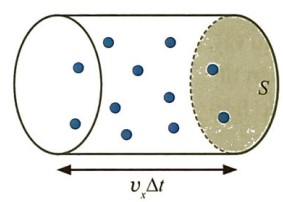
\includegraphics[width=0.3\linewidth]{../figs/VN12-Y24-PH-SYL-014-1}
				\captionof{figure}{Minh hoạ về các phân tử khí đập vào thành bình trong thời gian $\Delta t$.}
			\end{center}
			Gọi $\mu$ là mật độ phân tử khí. Xác định áp suất do các phân tử khí tác dụng lên thành bình theo $m$, $v_x$, $\mu$.
			\item Thực tế, các phân tử khí chuyển động hỗn loạn không có phương nào ưu tiên. Từ kết quả thu được ở câu b, em hãy mở rộng cho trường hợp chuyển động 3 chiều.
		\end{enumerate}
		
		
	}
	{\hide{\begin{enumerate}[label=\alph*)]
			\item Khi các phân tử khí chuyển động nhiệt đến va chạm vào thành bình sẽ gây ra áp suất lên thành bình. Áp suất này được tính bằng áp lực của các phân tử khí lên một đơn vị diện tích thành bình.\\
			Áp lực này càng lớn khi
			\begin{itemize}
				\item động lượng trước va chạm $m\vec{v}$ của các phân tử khí càng lớn $\Leftrightarrow m$ và $v$ càng lớn;
				\item số lượng phân tử khí va chạm với thành bình sau mỗi giây càng lớn $\Leftrightarrow$ mật độ phân tử khí $n$ càng lớn.
			\end{itemize}
			\item Sau khi va chạm với thành bình thì phân tử khí bị bật ngược trở lại với vận tốc $\vec{v}'_x$ với $v'_x=v_x$. Lực do thành bình tác dụng lên mỗi phân tử khí:
			$$\vec{f}_x=\dfrac{\Delta \vec{p}_x}{\Delta t}=\dfrac{m\left(\vec{v}'_x-\vec{v}_x\right)}{\Delta t}\Rightarrow f_x=\dfrac{2mv_x}{\Delta t}.$$
			Trong thời gian va chạm $\Delta t$, số phân tử đập vào diện tích $S$ của thành bình:
			$$N=\mu V=\mu Sv_x\Delta t.$$
			Do $N$ phân tử khí có thể chuyển động dọc trục $Ox$ theo hai chiều ngược nhau nên số lượng trung bình các phân tử khí đến đập vào diện tích $S$ của thành bình theo chiều dương gây áp suất lên thành $S$ là $\dfrac{N}{2}$.\\
			Tổng hợp lực do $\dfrac{N}{2}$ phân tử khí tác dụng lên thành bình theo chiều dương của trục $Ox$:
			$$F_x=\dfrac{N}{2}\cdot f_x=\dfrac{\mu Sv_x\Delta t}{2}\cdot\dfrac{2mv_x}{\Delta t}=\mu mv^2_xS.$$
			Áp suất do các phân tử khí tác dụng lên thành bình:
			$$p=\dfrac{F_x}{S}=\mu mv^2_x.$$
			\item Do phân tử khí chuyển động nhiệt theo cả ba phương và không có phương nào ưu tiên nên $v_x=v_y=v_z$:
			$$v^2=v^2_x+v^2_y+v^2_z=3v^2_x.$$
			Suy ra:
			$$p=\dfrac{1}{3}\mu mv^2.$$
			Vì ta đang xét chuyển động của nhiều phân tử khí nên $v^2$ là giá trị trung bình của bình phương tốc độ chuyển động nhiệt của từng phân tử. Khi đó:
			$$p=\dfrac{1}{3}\mu m\overline{v^2}.$$
		\end{enumerate}
	}}

	\viduii{2}
	{Thực nghiệm đo được tốc độ trung bình của hầu hết các phân tử khí trong khoảng từ vài trăm $\si{\meter/\second}$ đến vài ngàn $\si{\meter/\second}$. Tuy nhiên, phải sau một khoảng thời gian người ta mới cảm nhận được mùi thơm của lọ nước hoa bị đổ trong phòng. Hãy giải thích.
		
	}
	{\hide{Tốc độ trung bình trên một phương chỉ khoảng $\dfrac{1}{\sqrt{3}}\approx0,58 $ lần tốc độ chuyển động trung bình của phân tử khí. Mặt khác, do sự chuyển hỗn loạn và  trong quá trình khuếch tán, các phân tử nước hoa va chạm với các phân tử khí và các phân tử nước hoa khác làm lệch phương truyền. Do đó, cần nhiều thời gian hơn để các phân tử nước hoa có thể truyền đến được mũi người.
		
	}}
	
	\viduii{3}
	{Tính trung bình bình phương tốc độ trong chuyển động nhiệt của phân tử khí helium có khối lượng mol là $\SI{4}{\gram/\mole}$ ở nhiệt độ $\SI{320}{\kelvin}$. Coi các phân tử khí là giống nhau.
		
	}
	{\hide{Áp suất do khí tác dụng lên thành bình:
		\begin{eqnarray}
			&&p=\dfrac{1}{3}\mu m\overline{v^2}\nonumber\\
			&\Leftrightarrow& p=\dfrac{1}{3}\dfrac{N}{V}\cdot m\overline{v^2}\nonumber\\
			&\Leftrightarrow& pV=\dfrac{1}{3}Nm\overline{v^2} \label{eq:14.1}
		\end{eqnarray}
		Mà 
		\begin{equation}
			\label{eq:14.2}\\
			pV=n RT=\dfrac{Nm}{M}RT
		\end{equation}
		Thay (\ref{eq:14.2}) vào (\ref{eq:14.1}):
		$$\overline{v^2}=\dfrac{3RT}{M}=\dfrac{3\cdot\left(\SI{8.31}{\dfrac{\joule}{\mole\cdot\kelvin}}\right)\cdot\left(\SI{320}{\kelvin}\right)}{\SI{4E-3}{\kilogram/\mole}}=\SI{1.99E6}{\meter^2/\second^2}.$$
		
		
	}}
\end{dang}
\begin{dang}{Vận dụng được biểu thức tính động năng tịnh tiến trung bình của phân tử khí.}
	\viduii{2}
	{Tính nhiệt độ của một khối khí để động năng tịnh tiến trung bình trong chuyển động tịnh tiến của phân tử khí đó bằng $\SI{1.0}{\electronvolt}$. Lấy $\SI{1}{\electronvolt}=\SI{1.6E-19}{\joule}.$
		
	}
	{\hide{Nhiệt độ của khối khí:
		$$T=\dfrac{2}{3}\cdot\dfrac{W_\text{đ}}{k}=\dfrac{2}{3}\cdot\dfrac{\left(\SI{1.6E-19}{\joule}\right)}{\SI{1.38e-23}{\joule/\kelvin}}\approx\SI{7729.5}{\kelvin}.$$
		
	}}

	\viduii{2}
	{Xét khối khí chứa trong một bình kín, biết mật độ động năng phân tử (tổng động năng tịnh tiến của các phân tử khí trong $\SI{1}{\meter^3}$ thể tích khí) có giá trị $\SI{E-4}{\joule/\meter^3}$. Tính áp suất của khí trong bình.
		
	}
	{\hide{Mật độ động năng phân tử:
		$$\varepsilon=\dfrac{NW_\text{đ}}{V}=\mu W_\text{đ}=\SI{E-4}{\joule/\meter^3}.$$
		Áp suất của khí trong bình:
		$$p=\dfrac{NRT}{VN_A}=\mu kT$$
		$$\Rightarrow p=\dfrac{2}{3}\mu W_\text{đ}=\dfrac{2}{3}\varepsilon=\dfrac{2}{3}\cdot\left(\SI{E-4}{\joule/\meter^3}\right)=\SI{6.67E-5}{\pascal}.$$
		
	}}
\end{dang}
\begin{dang}{Nội năng khí lí tưởng \textit{(Đọc thêm)}}
\setcounter{section}{0}
\section{Nội năng khí lí tưởng đơn nguyên tử}
Đối với khí lí tưởng đơn nguyên tử, động năng chuyển động nhiệt của các phân tử khí chỉ gồm động năng chuyển động tịnh tiến. Do đó, nội năng của $\xsi{\nu}{\mole}$ khí lí tưởng đơn nguyên tử có dạng:
$$U=N\cdot\dfrac{3}{2}kT=\dfrac{3}{2}n N_\text{A}kT.$$
Thay $kN_\text{A}=R$, ta thu được:
$$U=\dfrac{3}{2}n RT.$$
Như vậy, nội năng của một khối khí lí tưởng xác định chỉ phụ thuộc nhiệt độ của khối khí.
\section{Công của khí thực hiện trong các đẳng quá trình}
Giả sử có $\xsi{n}{\mole}$ khí được chứa trong 1 cylanh cách nhiệt và được ngăn cách với bên ngoài bằng piston (tiết diện $S$) rất nhẹ, có thể trượt không ma sát trong cylanh. Khối khí dãn nở từ thể tích $V_1$ đến thể tích $V_2$. Xét trong từng quá trình thay đổi thể tích $dV$ rất bé, khối khí tác dụng lực $F=pS$ lên piston và đẩy nó trượt đoạn $dx$.\\
Công do khối khí thực hiện trong cả quá trình này:
$$A'=\int_{x_1}^{x_2} Fdx=\int_{x_1}^{x_2} pSdx=\int_{V_1}^{V_2}pdV.$$
Như vậy, độ lớn công của khối khí thực hiện bằng diện tích hình giới hạn bởi đồ thị $p\left(V\right)$ với trục hoành $OV$ trong khoảng $\left[V_1; V_2\right]$.\\
\begin{minipage}{0.45\textwidth}
	\subsection{Quá trình đẳng tích}
	\begin{center}
		\begin{tikzpicture} 
			\begin{axis}[line width=1pt,
				xmin=0,  
				xmax=3,  
				ytick={1,6},
				xtick={1},
				ymin=0,  
				ymax=7, 
				samples=300,
				yticklabels={$p_1$, $p_2$},
				xticklabels={$V_1$},
				axis lines=center, 
				xlabel=$V$, 
				ylabel=$p$, 
				every axis y label/.style={at=(current axis.above origin),anchor=south},  
				every axis x label/.style={at=(current axis.right of origin),anchor=west}]
				\draw[line width=0.5pt,blue, dashed] (axis cs: 1, 0) -- (axis cs: 1, 6);
				\draw[line width=0.5pt,blue, dashed] (axis cs: 1, 1) -- (axis cs: 0, 1);
				\draw[line width=0.5pt,blue, dashed] (axis cs: 1, 6) -- (axis cs: 0, 6);
				\draw[ultra thick,red] (axis cs: 1, 6) -- (axis cs: 1, 1);
				\draw[ultra thick,red,-latex] (axis cs: 1, 6) -- (axis cs: 1, 3);
				\filldraw[black] (axis cs:1,6) circle (1.5pt) node[right] {(1)};
				\filldraw[black] (axis cs:1,1) circle (1.5pt) node[right] {(2)};
			\end{axis}  
			\node[label={[below left]90:O}] at (0,0){};
		\end{tikzpicture}
	\end{center}
	Trong quá trình đẳng tích, khối khí không thay đổi thể tích nên:
	$$A'=0.$$
\end{minipage}
\begin{minipage}{0.1\textwidth}
	\
\end{minipage}
\begin{minipage}{0.45\textwidth}
	\subsection{Quá trình đẳng áp}
	\begin{center}
		\begin{tikzpicture} 
			\begin{axis}[ultra thick,
				xmin=0,  
				xmax=7,  
				ytick={6},
				xtick={1,6},
				ymin=0,  
				ymax=7, 
				samples=300,
				yticklabels={$p_1=p_2$},
				xticklabels={$V_1$, $V_2$},
				axis lines=center, 
				xlabel=$V$, 
				ylabel=$p$, 
				every axis y label/.style={at=(current axis.above origin),anchor=south},  
				every axis x label/.style={at=(current axis.right of origin),anchor=west}]
				\draw[line width=0.5pt,blue, dashed] (axis cs: 1, 0) -- (axis cs: 1, 6);
				\draw[line width=0.5pt,blue, dashed] (axis cs: 6, 6) -- (axis cs: 6, 0);
				\draw[line width=0.5pt,blue, dashed] (axis cs: 0, 6) -- (axis cs: 1, 6);
				\addplot[ultra thick, red, smooth, name path = f, domain=1:6] {6};
				\path[name path=xaxis]
				(\pgfkeysvalueof{/pgfplots/xmin},0) --
				(\pgfkeysvalueof{/pgfplots/xmax},0);
				\addplot[red!10, opacity=0.4] fill between[of=f and xaxis, soft clip={domain=1:6}];
				\addplot [ultra thick,-latex,red, smooth, domain=1:3.5] {6};  
				\filldraw[black] (axis cs:1,6) circle (1.5pt) node[above] {(1)};
				\filldraw[black] (axis cs:6,6) circle (1.5pt) node[above] {(2)};
			\end{axis}  
			\node[label={[below left]90:O}] at (0,0){};
		\end{tikzpicture}
	\end{center}
	Trong quá trình đẳng áp, do áp suất khí không đổi nên công do khí thực hiện:
	$$A'=p\Delta V.$$
\end{minipage}
\subsection{Quá trình đẳng nhiệt}
\begin{center}
	\begin{tikzpicture} 
		\begin{axis}[line width=1pt,
			xmin=0,  
			xmax=7,  
			ytick={1,6},
			xtick={1,6},
			ymin=0,  
			ymax=7, 
			samples=300,
			yticklabels={$p_1$, $p_2$},
			xticklabels={$V_1$, $V_2$},
			axis lines=center, 
			xlabel=$V$, 
			ylabel=$p$, 
			every axis y label/.style={at=(current axis.above origin),anchor=south},  
			every axis x label/.style={at=(current axis.right of origin),anchor=west}]
			\draw[line width=0.5pt,blue, dashed] (axis cs: 1, 0) -- (axis cs: 1, 6);
			\draw[line width=0.5pt,blue, dashed] (axis cs: 6, 0) -- (axis cs: 6, 1);
			\draw[line width=0.5pt,blue, dashed] (axis cs: 0, 6) -- (axis cs: 1, 6);
			\draw[line width=0.5pt,blue, dashed] (axis cs: 6, 1) -- (axis cs: 0, 1);
			\addplot[ultra thick, red, smooth, name path = f, domain=1:6] {6/x};
			\path[name path=xaxis]
			(\pgfkeysvalueof{/pgfplots/xmin},0) --
			(\pgfkeysvalueof{/pgfplots/xmax},0);
			\addplot[red!10, opacity=0.4] fill between[of=f and xaxis, soft clip={domain=1:6}];
			\addplot [ultra thick,-latex,red, smooth, domain=1:3] {6/x};  
			\filldraw[black] (axis cs:1,6) circle (1.5pt) node[above] {(1)};
			\filldraw[black] (axis cs:6,1) circle (1.5pt) node[above right] {(2)};
		\end{axis}  
		\node[label={[below left]90:O}] at (0,0){};
	\end{tikzpicture}
\end{center}
Công do khối khí thực hiện:
$$A'=\int_{V_1}^{V_2}pdV=n RT\int_{V_1}^{V_2}\dfrac{dV}{V}=n RT\ln\dfrac{V_2}{V_1}.$$
\section{Định luật I nhiệt động lực học}
$$\Delta U=Q+A=Q-A'$$
trong đó:
\begin{itemize}
	\item $\Delta U$: độ biến thiên nội năng của khối khí;
	\item $Q$: nhiệt lượng khí nhận;
	\item $A$: công khí nhận;
	\item $A'=-A$: công khí thực hiện.
\end{itemize}
\viduii{2}
{Một mol khí oxygen (giả thiết là khí lí tưởng) giãn nở ở nhiệt độ không đổi $T=\SI{310}{\kelvin}$ từ thể tích ban đầu $V_1=\SI{12}{\liter}$ tới thể tích cuối $V_2=\SI{19}{\liter}$. Công do khối khí thực hiện khi giãn nở là bao nhiêu?

}
{\hide{Công do khối khí thực hiện khi giãn nở ở nhiệt độ không đổi:
	$$A'=n RT\ln\dfrac{V_2}{V_1}=\left(\SI{1}{\mole}\right)\cdot\left(\SI{8.31}{\dfrac{\joule}{\mole\cdot\kelvin}}\right)\cdot\left(\SI{310}{\kelvin}\right)\cdot\ln\dfrac{\left(\SI{19}{\liter}\right)}{\left(\SI{12}{\liter}\right)}\approx\SI{1183}{\joule}.$$

}}

\viduii{3}{Có $\SI{6.5}{\gram}$ khí hydrogen ở $\SI{27}{\celsius}$ được đun nóng đẳng áp để thể tích tăng gấp đôi. Tính
	\begin{enumerate}[label=\alph*)]
		\item công do khí thực hiện.
		\item nhiệt lượng truyền cho khí.
		\item độ biến thiên nội năng của khí.
	\end{enumerate}
Biết nhiệt dung riêng đẳng áp của khí hydrogen là $c_p=\SI{14.3}{\kilo\joule/\kilogram\cdot \kelvin}$.
}
{\hide{\begin{center}
		\begin{tabular}{C{4cm} C{3cm} C{4cm}}
			\colorbox{green!40}{\textcolor{red}{\textbf{Trạng thái 1}}} & $\xrightarrow[]{p=\text{const}}$ & \colorbox{green!40}{\textcolor{red}{\textbf{Trạng thái 2}}}\\
			$V_1$ & & $V_2=2V_1$\\
			$T_1=\SI{300}{\kelvin}$ & & $T_2$
		\end{tabular}
	\end{center}
	\begin{enumerate}[label=\alph*)]
		\item Công do khí thực hiện:
		\begin{eqnarray*}
			&&A=p\Delta V=p\left(2V_1-V_1\right)=pV_1=\dfrac{m}{M}RT_1\\
			&\Rightarrow&A=\dfrac{\left(\SI{6.5}{\gram}\right)}{\left(\SI{2}{\gram/\mole}\right)}\cdot\left(\SI{8.31}{\dfrac{\joule}{\mole\cdot\kelvin}}\right)\cdot\left(\SI{300}{\kelvin}\right)=\SI{8.1}{\kilo\joule}.
		\end{eqnarray*}
		\item 		Trong quá trình đẳng áp:
		$$\dfrac{V_2}{V_1}=\dfrac{T_2}{T_1}\Rightarrow T_2=\dfrac{V_2}{V_1}T_1=2T_1.$$
		Nhiệt lượng truyền cho khí:
		\begin{eqnarray*}
			&&Q=mc_p\Delta T=mc_pT_1\\
			&\Rightarrow& Q=\left(\SI{6.5e-3}{\kilogram}\right)\cdot\left(\SI{14.3}{\kilo\joule/\kilogram\cdot\kelvin}\right)\cdot\left(\SI{300}{\kelvin}\right)\approx\SI{27.9}{\kilo\joule}.
		\end{eqnarray*}
\item Độ biến thiên nội năng của khí:
$$\Delta U=Q-A'=\SI{19.8}{\kilo\joule}.$$
		
	\end{enumerate}
}}
\end{dang}